\documentclass{article}
\setlength{\parindent}{0pt}
\setlength{\parskip}{2ex plus 0.5ex minus 0.2ex}
\usepackage[margin=1in]{geometry}
\usepackage{graphicx}
\usepackage{hyperref}
\usepackage{cleveref}
\usepackage{textcomp}
\usepackage{placeins}
\graphicspath{{./figures/}}

\title{Advanced Reactor Fuel cycle Molten Salt Reactor Design}
\author{Alexander Lindsay, Katy Huff} % As you author additions/changes, add
                                      % your name here!!!

\begin{document}
\maketitle

\section{Brief History}

The basis for this quick synopsis comes from
\cite{wiki:Molten_salt_reactor}. Research into molten salt reactors (MSRs) began
in earnest with the Aircraft Reactor Experiment (ARE), with experiments shared
between Oak Ridge National Lab (ORNL) and what is now Idaho National Lab
(INL). The ARE used NaF-ZrF$_4$-UF$_4$ (53-41-6 mol\%) as fuel. The reactor was
moderated by beryllium oxide (BeO), used liquid sodium as the secondary coolant,
and had a peak tempeature around 860 \textdegree C. The ARE managed to generate
100 MWh over the course of nine days in 1954. There was another reactor that
went critical at ORNL in 1957 called the Pratt and Whitney Aircraft Reactor-1
(PWAR-1). Although it produced essentially no power, the PWAR-1 is still one of
only three critical MSRs ever built.

The most successful MSR was the Molten-Salt Reactor Experiment (MSRE) which went
critical in 1965 and operated for four years at ORNL. The MSRE fuel was
LiF-BeF$_2$-ZrF$_4$-UF$_4$ (65-29-5-1 mol\%) with graphite core moderation. The
secondary coolant was 2LiF-BeF$_2$ (also known as FLiBe). Operating temperatures
went as high as 650 \textdegree C. MSRE neutronics were meant to mimic that of
an epithermal thorium molten salt breeder reactor (MSBR); however, for the MSRE
the expensive breeding blanket was sacrificed in favor of neutron
measurements. At full design power, the MSRE operated at 7.4 MW$_{th}$. Over the
course of the late 1960s the MSRE operated at full capacity for an equivalent of
1.5 years.

The logical follow-on from the MSRE was the MSBR; however, the MSBR was never
constructed. Funding for the MSR program was cut in favor of the liquid metal
fast-breeder reactor (LMFBR) program. Consequently, as of today, the ARE,
PWAR-1, and MSRE are the only critical MSRs ever operated.

\section{Comprehensive, expensive (3D) models}

\subsection{MSRE}

\subsection{MSBR}

The most detailed report on ORNL's molten salt breeder reactor is the technical
report by Robertson. \cite{robertson_conceptual_1971} A nice overview of the
MSBR geometry is shown in \cref{fig:vertical,fig:horizontal,fig:zoom_horiz}.

\begin{figure}[htpb]
  \centering
  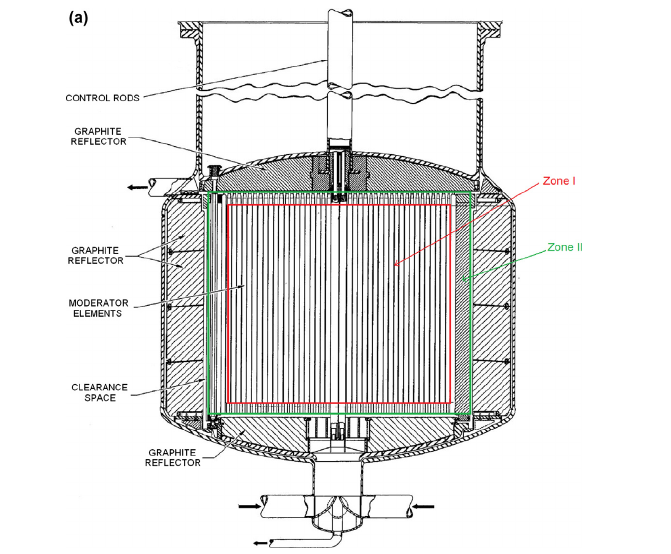
\includegraphics{vertical_MSBR_cross_section.png}
  \caption{Vertical cross section of MSBR.}
  \label{fig:vertical}
\end{figure}
\begin{figure}[htpb]
  \centering
  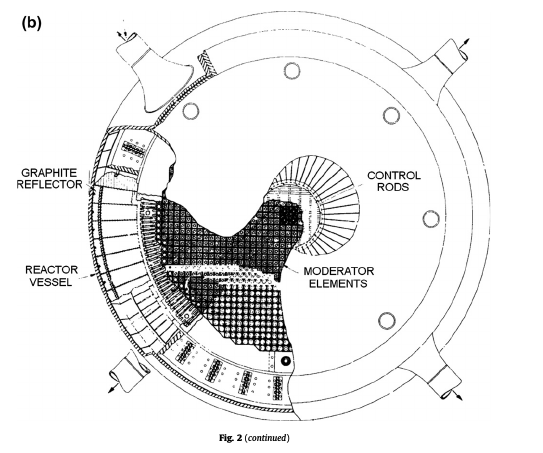
\includegraphics{horizontal_MSBR_cross_section.png}
  \caption{Horizontal cross section of MSBR.}
  \label{fig:horizontal}
\end{figure}
\begin{figure}[htpb]
  \centering
  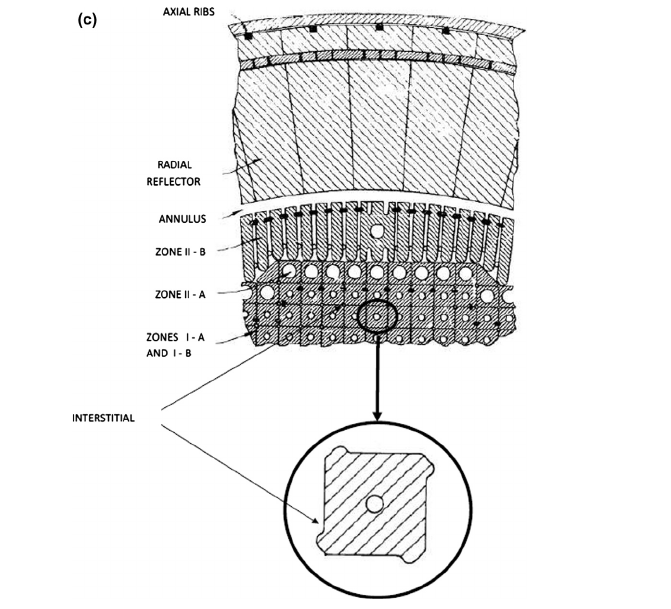
\includegraphics{zoomed_horizontal_MSBR_cross_section.png}
  \caption{Zoomed in horizontal cross-section of MSBR. Shows presence of
    interstitials between graphite block elements in zone 1 of the reactor.}
  \label{fig:zoom_horiz}
\end{figure}

\section{Simplified models}

\subsection{MSBR children}

\subsubsection{Cammi et. al.}

This model is based on the multi-physics model by
\cite{cammi_multi-physics_2011}.

\FloatBarrier

\bibliographystyle{unsrt}
\bibliography{MSR-design}
\end{document}
